\documentclass[hidelinks, a4paper, 12pt]{article}
\usepackage[linktoc=all]{hyperref}
\usepackage{apacite}
\usepackage[margin=1.0in]{geometry}
\usepackage{amssymb}
\usepackage{amsmath}
\usepackage{amsthm}
\usepackage{tikz}
\usepackage{pgf}
\usepackage{mathrsfs}
\usepackage{array}
\usepackage{tabularx}

\allowdisplaybreaks

\hypersetup{
    pdftitle={Pure Mathematics I: Differentiation},
    pdfauthor={Wilson Wongso},
    pdfpagemode=UseOutlines,
}

\title{Pure Mathematics I: Differentiation}
\author{Based on lectures by Danilo J. Alcordo \\ Notes taken by Wilson Wongso}
\date{Junior College 1 - Academic Year 2017/2018}

\setcounter{section}{-1}
\setcounter{tocdepth}{2}

\graphicspath{ {./images/} }

\newcommand{\biimp}{\Leftrightarrow}
\newcommand{\bd}{\textbf}
\newcommand{\n}{\\[\baselineskip]}
\newcommand{\real}{\mathbb{R}}
\newcommand{\thus}{\Rightarrow}

\begin{document}
    
    \maketitle
        
    \tableofcontents

    \section{Preface}
        The following lecture notes are mostly based on textbook \cite{neill2016cambridge} questions. The author assumes the readers understands basic coordinate geometry.\\[\baselineskip]
        These notes only include the key parts of the lectures and the types of problems that often appear in the actual exam.
        Further reading and past-year papers practice are highly encouraged.

    \section{Gradient}
        In the previous topic of coordinate geometry, we are able to find the gradient of a straight line by the idea of finding the change in rise ($y$) over the
        change in run ($x$), usually in the form of:
        \[m = \frac{\Delta y}{\Delta x}\]
        Now, what happens if we would like to find the gradient of a non-straight line? How can we mathematically describe their gradients?\n
        The solution to this is by differentiation, from which we can find the expression (the derivative) which describes the gradient of any kind of lines, given that we know its equation.

    \section{Introduction to Derivatives}
        The method for finding a derivative actually comes from its formal definition, although usually it is rarely proven where these methods and techniques are derived from.\n
        Furthermore, derivatives are also based off the concept of limits, which yet again is not part of the curriculum (sadly). To put simply, we can say that a limit is the value 
        that a function "approaches" as the input "approaches" some value. \cite{stewart2007calculus}\n
        With that aside, let's see what the formal definition of a derivative is.

        \subsection{Definition of a Derivative}
            The \bd{derivative} of a function $f$ is a function denoted by $f'(x)$ such that its value at a number $x$ in the domain of $f$ is given by:
            \[f'(x) = \lim_{h\to0} \frac{f(x+h)-f(x)}{h}\]
            A lot of new notations for sure, but we'll try to see its geometric representation, which hopefully would help visualize derivatives.

        \subsection{Geometric Representation of a Derivative}
            The blue line in the graph below represents the function $f(x)$ and we would like to find its derivative at the point $x$, denoted by the red dot.
            \begin{figure}[ht]
                \centering
                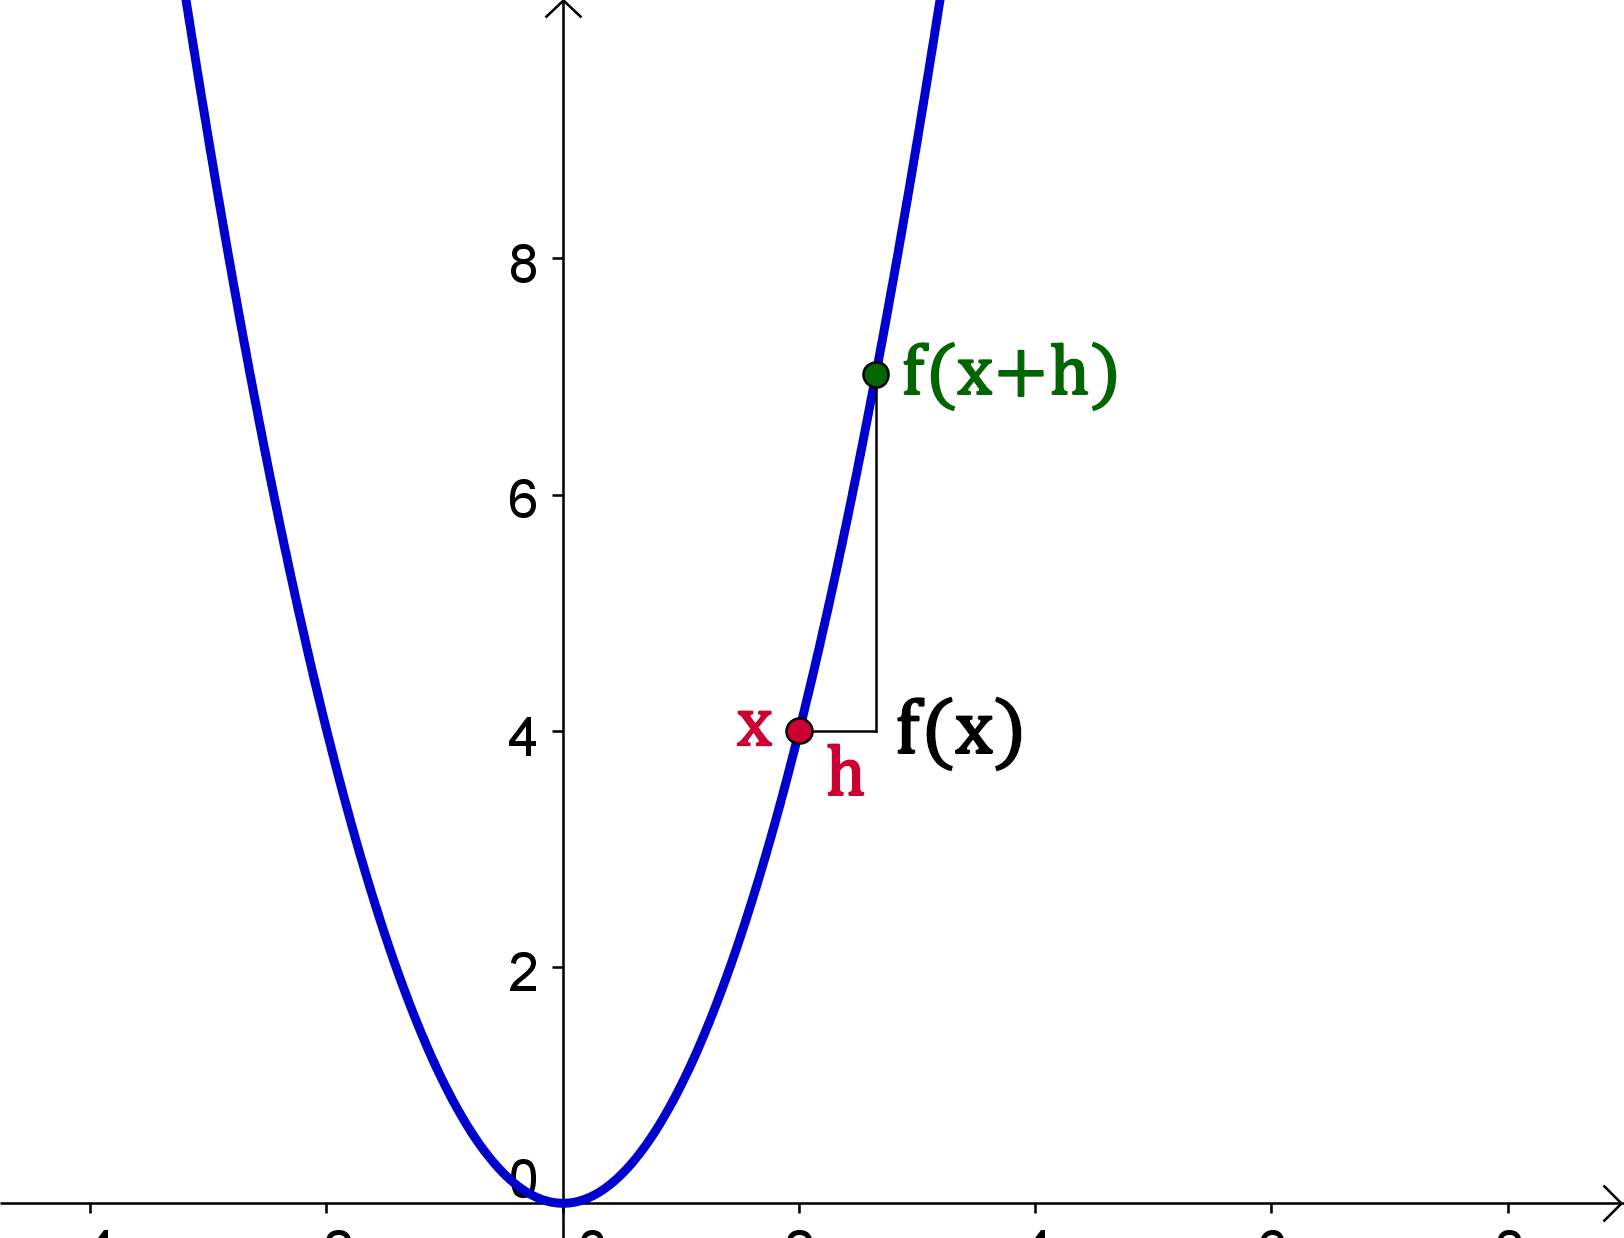
\includegraphics[scale=0.15]{derivative}
            \end{figure}\n
            Similar to the equation found in section \bd{1 Gradient}, we need to find the change in $y$ over the change in $x$, and we do that by finding another point that is close enough to
            the point $x$, in this case a small change denoted by $h$. As we decrease $h$ to $0$, we can then find the gradient simply by the equation:
            \[m = \frac{\Delta y}{\Delta x} = \frac{f(x+h)-f(x)}{h}\]
            Since we want $h$ to approach zero, or take the smallest value possible, we then need to find the limit as $h$ approaches zero, which then brings us back to the equation:
            \[f'(x) = \lim_{h\to0} \frac{f(x+h)-f(x)}{h}\]
            Hopefully this representation makes more sense for what a derivative actually is -- slope of a line.
        
        \subsection{Notations of a Derivative}
            A small yet important reminder, there are multiple ways to annotate a derivative. For instance,
            \[f'(x)\]
            is Lagrange's notation, read as 'f prime'. Higher order derivatives will simply append more primes to $f$, such that the second derivative of $f$ is
            \[f''(x)\]
            and so on.\n
            Otherwise, there is also Leibniz's notation when the equation $y = f(x)$ is viewed as a functional relationship between dependent and independent variables. 
            Then the first derivative is denoted by
            \[\frac{dy}{dx}\]
            and its second derivative
            \[\frac{d^2y}{dx^2}\]
            Hence higher order derivatives are denoted by
            \[\frac{d^ny}{dx^n}\]

    \section{Limits}
        Although not part of the curriculum, there are some theorems and practice questions regarding limits given by the lecturer. This would later be useful 
        as we can then use the formal definition of a derivative to differentiate a function, without memorizing different theorems on differentiation.
        \subsection{Theorems of Limits}
            \subsubsection{Limit of the Identity Function}
                \[\lim_{x\to a} x = a\]

            \subsubsection{Limit of a Constant}
                If $c$ is a constant, then $\forall c \in \mathbb{R}$
                \[\lim_{x\to a} c = c\]

            \subsubsection{Limit of a Linear Function}
                If $m$ and $b$ are constants
                \[\lim_{x\to a} (mx+b) = ma + b\]

            \subsubsection{Limit of the Sum and Difference of Two Functions}
                If $\lim_{x\to a}f(x) = L$ and $\lim_{x\to a}g(x) = M$, then
                \[\lim_{x\to a} [f(x)\pm g(x)] = L \pm M\]

            \subsubsection{Limit of the Product of Two Functions}
                If $\lim_{x\to a}f(x) = L$ and $\lim_{x\to a}g(x) = M$, then
                \[\lim_{x\to a} [f(x)\cdot g(x)] = L \cdot M\]

            \subsubsection{Limit of the Quotient of Two Functions}
                If $\lim_{x\to a}f(x) = L$ and $\lim_{x\to a}g(x) = M$, then
                \[\lim_{x\to a} \frac{f(x)}{g(x)} = \frac{L}{M}, M \neq 0\]

            \subsubsection{Limit of the n\textsuperscript{th} Root of a Function}
                If $a$ is a positive integer and $\lim_{x\to a}f(x) = L$, then
                \[\lim_{x\to a} \sqrt[\leftroot{-2}\uproot{2}n]{f(x)} = \sqrt[\leftroot{-2}\uproot{2}n]{L}\]
                with the restriction that if $n$ is even, $L > 0$.

        \subsection{Example Problems}
            \subsubsection{Problem 1}
                Find the limit of the following functions
                \begin{center}
                    \begin{tabularx}{\textwidth} {
                        X X X}
                        (a) $\lim_{x\to2} 7$ & (b) $\lim_{x\to2} (2x+1)$ & (c) $\lim_{x\to0} (2x^2 - 5x + 1)$\\ 
                        \\
                        (d) $\lim_{x\to2} x$  & (e) $\lim_{x\to1} \frac{3x-1}{2x+6}$  & (f) $\lim_{x\to-6} \frac{x^2+4x-12}{x+6}$ \\  
                        \\
                        (g) $\lim_{x\to25} \frac{2x-50}{\sqrt{x}-5}$
                    \end{tabularx}
                \end{center}
                \bd{Solution}\n
                \bd{(a)} Use limit of a constant,
                \[\lim_{x\to2} 7 = 7\]
                \bd{(b)}Use limit of a linear function,
                \[\begin{split}
                    \lim_{x\to2} (2x+1) &= (2\cdot2) + 1\\
                    &= 4+ 1\\
                    &=5
                \end{split}\]
                \bd{(c)} Use limit of sum of functions,
                \[\begin{split}
                    \lim_{x\to0} (2x^2 - 5x + 1) &= 2\cdot(0)^2 - (5\cdot 0) + 1\\
                    &= 0 + 0 + 1\\
                    &= 1
                \end{split}\]
                \bd{(d)} Use limit of the identity function,
                \[\lim_{x\to2} x = 2\]
                \bd{(e)} Use limit of quotient of two functions,
                \[\begin{split}
                    \lim_{x\to1} \frac{3x-1}{2x+6} &= \frac{(3\cdot1) - 1}{(2\cdot 1) + 6}\n
                    &= \frac{3-1}{2+6}\n
                    &= \frac{2}{8}\n
                    &= \frac{1}{4} 
                \end{split}\]
                \bd{(f)} Using the limit of quotient of two functions would make the denominator equal to zero, which is restricted. Instead, 
                we should first manipulate the equation, as follows.
                \[\begin{split}
                    \lim_{x\to -6} \frac{x^2+4x-12}{x+6} &= \lim_{x\to -6} \frac{(x+6)(x-2)}{(x+6)}\n
                    &= \lim_{x\to -6} (x-2)\n
                    &= -6 - 2\n
                    &= -8 
                \end{split}\]
                \bd{(g)} Similarly, using the limit of quotient of two functions would make the denominator equal to zero. To solve the limit, we
                can multiply the equation by the conjugate of the denominator, as so:
                \[\begin{split}
                    \lim_{x\to 25} \frac{2x-50}{\sqrt{x}-5} &= \lim_{x\to 25} \frac{2x-50}{\sqrt{x}-5} \cdot \frac{\sqrt{x}+5}{\sqrt{x}+5}\n
                    &= \lim_{x\to 25} \frac{(2x-50)(\sqrt{x}+5)}{x-25}\n
                    &= \lim_{x\to 25} \frac{2(x-25)(\sqrt{x}+5)}{x-25}\n
                    &= \lim_{x\to 25} 2(\sqrt{x}+5)\n
                    &= \lim_{x\to 25} (2\sqrt{x}+10)\n
                    &= (2\cdot \sqrt{25}) + 10\n
                    &= (2 \cdot 5) + 10\n
                    &= 10 + 10\n
                    &= 20
                \end{split}\]
    
            \subsubsection{Problem 2}
                Find the derivative of following functions
                \begin{center}
                    \begin{tabularx}{\textwidth} {
                        X X X}
                        (a) $f(x) = 3x-7$ & (b) $g(x) = x^2-4$ & (c) $h(x) = 3x^2+9x-6$\\ 
                        \\
                        (d) $y = \frac{x^2-1}{x+1}$  & (e) $g(x) = (x-8)(x+5)$\\  
                    \end{tabularx}
                \end{center}
                \medskip
                \bd{Solution}\n
                To solve, we can utilize the definition of a derivative using limits, i.e.
                \[f'(x) = \lim_{h\to0} \frac{f(x+h)-f(x)}{h}\]
                \bd{(a)}
                \[\begin{split}
                    f(x) &= 3x-7\n
                    f'(x) &= \lim_{h\to0}\frac{[3(x+h)-7] - (3x-7)}{h}\n 
                    f'(x) &= \lim_{h\to0}\frac{3x + 3h - 7 - 3x + 7}{h}\n
                    f'(x) &= \lim_{h\to0}\frac{3h}{h}\n
                    f'(x) &= 3           
                \end{split}\]
                \n\bd{(b)}
                \[\begin{split}
                    g(x) &= x^2-4\n
                    g'(x) &= \lim_{h\to0}\frac{[(x+h)^2-4] - (x^2-4)}{h}\n 
                    g'(x) &= \lim_{h\to0}\frac{x^2 +2xh + h^2 - 4 - x^2 + 4}{h}\n
                    g'(x) &= \lim_{h\to0}\frac{2xh + h^2}{h}\n
                    g'(x) &= \lim_{h\to0}\frac{h(2x + h)}{h}\n
                    g'(x) &= \lim_{h\to0}(2x+h)\n
                    g'(x) &= 2x           
                \end{split}\]
                \n\bd{(c)}
                \[\begin{split}
                    h(x) &= 3x^2+9x-6\n
                    h'(x) &= \lim_{h\to0}\frac{[3(x+h)^2+9(x+h)-6] - (3x^2+9x-6)}{h}\n
                    h'(x) &= \lim_{h\to0}\frac{3(x^2+2xh+h^2)+9x+9h-6-3x^2-9x+6}{h}\n
                    h'(x) &= \lim_{h\to0}\frac{3x^2+6xh+3h^2+9x+9h-6-3x^2-9x+6}{h}\n
                    h'(x) &= \lim_{h\to0}\frac{6xh+3h^2+9h}{h}\n
                    h'(x) &= \lim_{h\to0}\frac{h(6x+3h+9)}{h}\n
                    h'(x) &= \lim_{h\to0}(6x+3h+9)\n
                    h'(x) &= 6x+9           
                \end{split}\]
                \n\bd{(d)}
                \[\begin{split}
                    y &= \frac{x^2-1}{x+1}\n
                    y &= \frac{(x+1)(x-1)}{(x+1)}\n
                    y &= x-1\n
                    y' &= \lim_{h\to0}\frac{[(x+h)-1] - (x-1)}{h}\n 
                    y' &= \lim_{h\to0}\frac{x+h-1 -x+1}{h}\n 
                    y' &= \lim_{h\to0}\frac{h}{h}\n 
                    y' &= 1\n 
                \end{split}\]
                \n\bd{(e)}
                \[\begin{split}
                    g(x) &= (x-8)(x+5)\n
                    g(x) &= x^2-3x-40\n
                    g'(x) &= \lim_{h\to0}\frac{[(x+h)^2-3(x+h)-40] - (x^2-3x-40)}{h}\n 
                    g'(x) &= \lim_{h\to0}\frac{x^2+2xh+h^2-3x-3h-40-x^2+3x+40}{h}\n 
                    g'(x) &= \lim_{h\to0}\frac{2xh+h^2-3h}{h}\n 
                    g'(x) &= \lim_{h\to0}\frac{h(2x+h-3)}{h}\n 
                    g'(x) &= \lim_{h\to0}(2x+h-3)\n 
                    g'(x) &= 2x-3       
                \end{split}\]
    
    \section{Differentiation}
        \subsection{Theorems of Differentiation}
            Now, it's clearly tiresome to keep on using the formal definition of a derivative, but there are theorems of differentiation
            that would ease us in finding derivatives. Fear not of memorization, since they are given in the formula sheet during the exam.
            \subsubsection{Constant Rule}
                If $f(x) = c, \forall x \in \real,$ then
                \[f'(x) = 0\]
            \subsubsection{Power Rule}
                If $f(x) = x^n,$ then
                \[f'(x) = nx^{n-1}\]
            \subsubsection{Constant Multiple Rule}
                If $g(x) = c\cdot f(x),$ then
                \[g'(x) = c\cdot f'(x)\]
            \subsubsection{Sum Rule}
                If $h(x) = f(x) + g(x),$ then
                \[h'(x) = f'(x) + g'(x)\]
            \subsubsection{Difference Rule}
                If $h(x) = f(x) - g(x),$ then
                \[h'(x) = f'(x) - g'(x)\]
            \subsubsection{Product Rule}
                If $f(x) = u\cdot v,$ then
                \[f'(x) = udv + vdu\]
            \subsubsection{Quotient Rule}
                If $f(x) = \frac{u}{v},$ then
                \[f'(x) = \frac{vdu - udv}{v^2}\]
            \subsubsection{Chain Rule}
                If $f(x) = f(g(x)),$ then
                \[f'(x) = f'(g(x))\cdot g'(x)\]
        \subsection{Example Problems}
            \subsubsection{Problem 1}
                Differentiate the following functions:
                \begin{center}
                    \begin{tabularx}{\textwidth} {
                        X X X}
                        (a) $y = x(1+x^2)$ & (b) $y = (1+\sqrt{x})^2$ & (c) $y = \frac{x^2+x+1}{x}$\\ 
                        \\
                        (d) $y = x - \frac{1}{2}\sqrt{x}$  & (e) $y = x(1-\frac{1}{\sqrt{x}})$ & (f) $y = x - \frac{1}{x}$\\
                        \\
                        (g) $y = (x^3-2)^3$
                    \end{tabularx}
                \end{center}
                \medskip
                \bd{Solution}\n
                \bd{(a)} Distribute $x$ and use the power rule.
                \[\begin{split}
                    y &= x(1+x^2)\\
                    y &= x+x^3\\
                    y &= x^1 + x^3\\
                    y' &= 1(x)^0 + 3(x)^2\\
                    y' &= 1+3x^2 
                \end{split}\]
                \bd{(b)} Use both power rule and chain rule.
                \[y = (1+\sqrt{x})^2\]
                We can let $u$ be the equation inside the square function,
                \[\begin{split}
                    u &= 1+\sqrt{x}\\
                    u &= 1 + x^{\frac{1}{2}}\\
                    u' &= \frac{1}{2}(x)^{-\frac{1}{2}}\\
                    u' &= \frac{1}{2\sqrt{x}}
                \end{split}\]
                Then by the chain rule,
                \[\begin{split}
                    y' &= 2(1+\sqrt{x})\left(\frac{1}{2\sqrt{x}}\right)\\
                    y' &= \frac{1+\sqrt{x}}{\sqrt{x}}
                \end{split}\]\n
                \bd{(c)} Use the quotient rule.
                \[y = \frac{x^2+x+1}{x}\]
                Set $u$ as the numerator,
                \[\begin{split}
                    u &= x^2 + x + 1\\
                    du &= 2x + 1
                \end{split}\]
                And $v$ as the denominator,
                \[\begin{split}
                    v &= x\\
                    dv &= 1
                \end{split}\]
                Hence the derivative,
                \[\begin{split}
                    y' &= \frac{vdu-udv}{v^2}\\
                    y' &= \frac{x(2x + 1)-(x^2 + x + 1)}{x^2}\\
                    y' &= \frac{2x^2+x-x^2-x-1}{x^2}\\
                    y' &= \frac{x^2-1}{x^2}
                \end{split}\]
                \bd{(d)} Use the power rule.
                \[\begin{split}
                    y &= x - \frac{1}{2}\sqrt{x}\\
                    y &= x - \frac{1}{2}(x)^{\frac{1}{2}}\\
                    y' &= 1 - \frac{1}{2}\cdot \frac{1}{2}(x)^{-\frac{1}{2}}\\
                    y' &= 1 - \frac{1}{4\sqrt{x}}
                \end{split}\]
                \bd{(e)} Distribute $x$ and use the power rule.
                \[\begin{split}
                    y &= x\left(1-\frac{1}{\sqrt{x}}\right)\\
                    y &= x - \frac{x}{\sqrt{x}}\\
                    y &= x - \frac{x}{x^{\frac{1}{2}}}\\
                    y &= x - x^{\frac{1}{2}}\\
                    y' &= 1 - \frac{1}{2}(x)^{-\frac{1}{2}}\\
                    y' &= 1 - \frac{1}{2\sqrt{x}}
                \end{split}\]
                \bd{(f)} Use the power rule.
                \[\begin{split}
                    y &= x - \frac{1}{x}\\
                    y &= x - x^{-1}\\
                    y' &= 1 -(-1)x^{-2}\\
                    y' &= 1+\frac{1}{x^2}
                \end{split}\]
                \bd{(g)} Use the power rule and chain rule.
                \[y = (x^3-2)^3\]
                We can let $u$ be the equation inside the cube function,
                \[\begin{split}
                    u &= x^3-2\\
                    u' &= 3x^2
                \end{split}\]
                Then by the chain rule,
                \[\begin{split}
                    y' &= 3(x^3-2)^2\cdot(3x^2)\\
                    y' &= 9x^2\cdot(x^3-2)^2
                \end{split}\]
    
    \section{Tangents and Normals of Graphs}
        Now that we know how to find derivatives, we can relate them with graphs, since they correspond to the graph's
        gradient.
        \subsection{Gradient of a Tangent}
            Given a function $y$, and given a point $x$, we can find the gradient $m$ of the tangent of the graph at the given point $x$ such that,
            \[m = y'(x)\]

        \subsection{Normal to a Tangent of a Graph}
            Since we can find the gradient $m$ of the tangent of a graph, the normal $m_{\perp}$ (perpendicular gradient) to that tangent is given by:
            \[m_{\perp} \biimp -\frac{1}{m} \biimp -\frac{1}{y'(x)}\]
        
        \subsection{Example Problems}
            \subsubsection{Problem 1}
                Find the gradient of the tangent to the graph of $y = x^2$ at $x = -3.5$.\n
                \bd{Solution}\n
                Find the derivative of the function.
                \[\begin{split}
                    y &= x^2\\
                    y' &= 2x\\
                \end{split}\]
                Plug the value of $x$ into $y'$:
                \[\begin{split}
                    m &= y'(x)\\
                    m &= 2(-3.5)\\
                    m &= -7
                \end{split}\]
            \subsubsection{Problem 2}
            Find the gradient of the tangent to the graph of $y = x^3$ at $x = 2$.\n
            \bd{Solution}\n
            Find the derivative of the function.
            \[\begin{split}
                y &= x^3\\
                y' &= 3x^2\\
            \end{split}\]
            Plug the value of $x$ into $y'$:
            \[\begin{split}
                m &= y'(x)\\
                m &= 3(2)^2\\
                m &= 3(4)\\
                m &= 12
            \end{split}\] 

    \section{Tangents and Normals as Essay Questions}
        In the exam, what the question requires from us don't appear explicitly. Often, we need to first find out what it
        requires, and take steps to reach it. The key to mastering these kinds of question is again, practice.\n
        \bd{\textit{Author's Note: }}Practice will surely pay off, at least in Pure Mathematics :)

        \subsection{Example Problems}
            \subsubsection{Problem 1}
                Find the equation of the tangent to the graph $y = x^2 + 2$ where $x = -1$.\n
                \bd{Solution}\n
                Firstly, we need to find the coordinate of $y$, with the given point $x$:
                \[\begin{split}
                    y &= x^2+2\\
                    y &= (-1)^2+2\\
                    y &= 1+2\\
                    y &= 3
                \end{split}\]
                Obtaining the coordinate $(-1, 3)$.\n
                Then, we need to find the gradient of the tangent, i.e. derivative at $x = -1$:
                \[\begin{split}
                    y &= x^2 + 2\\
                    y' &= 2x
                \end{split}\]
                Plug the value of $x$ into $y'$ yields:
                \[\begin{split}
                    m &= 2(-1)\\
                    m &= -2
                \end{split}\]
                With that, we can find the equation of the tangent, using the same equation found in coordinate geometry:
                \[y-y_0 = m(x-x_0)\]
                where $m$ is the gradient and $(x_0, y_0)$ is the set of coordinates of a point that lies on the line.\n
                Therefore at $m = -2$ and $(-1, 3)$, the equation of the tangent line is:
                \[\begin{split}
                    y - 3 &= -2(x-(-1))\\
                    y - 3 &= -2(x+1)\\
                    y - 3 &= -2x -2\\
                    y & = -2x +1
                \end{split}\]
                \bd{Notice: }The steps to accomplish the task are as follows:\n
                $\bullet$ Find the \bd{coordinates} of the point that lies on the tangent line.\n
                $\bullet$ Find the \bd{derivative} of the function, and plug the value of $x$ to find the \bd{gradient}.\n
                $\bullet$ Construct the \bd{equation of tangent line} using the equation $y-y_0 = m(x-x_0)$ with the corresponding
                values found in the steps above.
            
            \subsubsection{Problem 2}
                Find the equation of the normal to the graph $y = x^2 + 1$ where $x = 0$.\n
                \bd{Solution}\n
                As mentioned in the last part of \bd{6.1.1 Problem 1}, we can finish the task by the same step, although with a slight
                difference.\n
                $\bullet$ Coordinate of $y$ at $x = 0$:
                \[\begin{split}
                    y &= x^2 + 1\\
                    y &= (0)^2 + 1\\
                    y &= 1
                \end{split}\]
                Obtaining $(0, 1)$.\n
                $\bullet$ Gradient at $x = 0$:\n
                Find the derivative:
                \[\begin{split}
                    y &= x^2 + 1\\
                    y' &= 2x
                \end{split}\]
                Plug in the value of $x$:
                \[\begin{split}
                    m &= 2(0)\\
                    m &= 0
                \end{split}\]
                Since we are looking for the equation of the normal, then we need to find the gradient perpendicular to $m$, denoted by $m_\perp$:
                \[\begin{split}
                    m_{\perp} &= -\frac{1}{m}\\
                    m_{\perp} &= -\frac{1}{0}\\
                \end{split}\]
                Such gradient is an indeterminate form, but we do know that such gradient belongs to a straight, vertical line of the form:
                \[x = a\]
                where $a$ is the point at which the line crosses the $x$-axis.\n
                We do know that the line passes through $(0, 1)$, thus it crosses the $x$-axis at $x = 0$.\n
                Hence the equation of the normal is given by:
                \[x = 0\]

            \subsubsection{Problem 3}
                The tangent $P$ to the curve $y = x^2$ has gradient $-1$. Find the equation of the normal at $P$.\n
                \bd{Solution}\n
                Unlike the previous problems, we need to work backwards this time. Because we have the value of the gradient, we just need the coordinates at which 
                the tangent has gradient $-1$.\n
                First, find the derivative:
                \[\begin{split}
                    y &= x^2\\
                    y' &= 2x
                \end{split}\]
                Then, equate $y'$ to the gradient:
                \[\begin{split}
                    -1 &= 2x\\
                    x &= -\frac{1}{2}
                \end{split}\]
                Find the coordinate of $y$ at the corresponding $x$:
                \[\begin{split}
                    y &= x^2\\
                    y &= \left(-\frac{1}{2}\right)^2\\
                    y &= \frac{1}{4}\\
                \end{split}\]
                Obtaining the coordinate $P = \left(-\frac{1}{2}, \frac{1}{4}\right)$.\n
                Then, because the question wants the equation of the normal, we need to find the perpendicular gradient:
                \[\begin{split}
                    m_\perp &= -\frac{1}{m}\\
                    m_\perp &= -\frac{1}{(-1)}\\
                    m_\perp &= 1
                \end{split}\]
                Finally we can find the equation of the normal at $P$:
                \[\begin{split}
                    y-y_0 &= m(x-x_0)\n
                    y-\frac{1}{4} &= x - \left(-\frac{1}{2}\right)\n
                    y-\frac{1}{4} &= x +\frac{1}{2}\n
                    y &= x + \frac{3}{4}
                \end{split}\]
            
            \subsubsection{Problem 4}
                Find the equation of the tangent to the curve $y = x^2 -2x$ which is perpendicular to the line $2y = x -1$.\n
                \bd{Solution}\n
                Unlike \bd{6.1.3 Problem 3}, the gradient is not explicitly given by the question, thus more work needs to be done.
                We can obtain it by finding the gradient of the line $2y = x - 1$.
                \[\begin{split}
                    2y &= x - 1\\
                    y &= \frac{1}{2}x - \frac{1}{2}
                \end{split}\]
                since the line above is perpendicular to the tangent, we can denote its gradient with $m_\perp$:
                \[\begin{split}
                    m_\perp &= \frac{1}{2}\\
                    \Rightarrow m &= -2\\
                \end{split}\]
                Now that we've obtained the gradient, we can find the coordinate at which the tangent has the gradient of $-2$.\n
                We can first derive the function $y = x^2 - 2x$:
                \[\begin{split}
                    y &= x^2 - 2x\\
                    y' &= 2x - 2
                \end{split}\]
                Then equate $y'$ to the gradient $m$ to find the point $x$:
                \[\begin{split}
                    -2 &= 2x - 2\\
                    0 &= 2x\\
                    x &= 0
                \end{split}\]
                Find the $x$ coordinate, we can find the corresponding $y$ coordinate by plugging the value of $x$ into $y$:
                \[\begin{split}
                    y &= x^2 - 2x\\
                    y &= (0)^2 - 2(0)\\
                    y &= 0
                \end{split}\]
                Therefore the point has the coordinate $(0, 0)$.\n
                Finally, we can construct the equation of the tangent:
                \[\begin{split}
                    y - y_0 &= m (x-x_0)\\
                    y - 0 &= -2(x-0)\\
                    y &= -2x
                \end{split}\]
            \subsubsection{Problem 5}
                Find the equation of the normal to the curve $y = (x-1)^2$ which is parallel to the $y$-axis.\n
                \bd{Solution}\n
                Similarly, we need to do work to find the gradient of the normal.\n
                We begin by differentiating the function $y = (x-1)^2$ using the chain rule:
                \[\begin{split}
                    y &= (x-1)^2\\
                    y' &= 2(x-1) \cdot 1\\
                    y' &= 2x - 2
                \end{split}\]
                Because $y'$ corresponds to the gradient of the tangent, we need to find the expression which corresponds
                to the gradient of the normal instead.
                \[\begin{split}
                    m &= y'\\
                    m &= 2x - 2\\
                    \thus m_\perp &= -\frac{1}{2x-2}
                \end{split}\]
                The question states that the normal is parallel to the $y$-axis, whose gradient we know is:
                \[m_{y-axis} = \frac{1}{0}\]
                Then we can simply equate it to $m_\perp$:
                \[\begin{split}
                    m_{y-axis} &= m_\perp\\
                    \frac{1}{0} &= -\frac{1}{2x-2}\\
                \end{split}\]
                Looking at the equation above, we can equate the respective denominators to each other.
                \[\begin{split}
                    0 &= 2x-2\\
                    2x &= 2\\
                    x &= 1
                \end{split}\]
                With the point $x=1$, we can finally say that the equation of normal is simply:
                \[x = 1\]
                because it is parallel to thee $y$-axis and crosses the $x$-axis at $x = 1$.
            \subsubsection{Problem 6}
                The tangent to the curve $y = 6\sqrt{x}$ at the point $(4, 12)$ meets the axes at $A$ and $B$. 
                Show that the distance $AB$ may be written in the form $k\sqrt{13}$, and state the value of $k$.\n
                \bd{Solution}\n
                The question gave us the coordinate for the tangent, so we only need to find the gradient in order to find the 
                equation of the tangent line.
                \[\begin{split}
                    y &= 6\sqrt{x}\\
                    y &= 6(x)^{\frac{1}{2}}\\
                    y' &= 6\cdot\left(\frac{1}{2}x^{-\frac{1}{2}}\right)\\
                    y' &= 3x^{-\frac{1}{2}}\\
                    y' &= \frac{3}{\sqrt{x}}
                \end{split}\]
                At the point $(4, 12)$, the gradient has a value of:
                \[\begin{split}
                    m &= \frac{3}{\sqrt{x}}\\
                    m &= \frac{3}{\sqrt{4}}\\
                    m &= \frac{3}{2}
                \end{split}\]
                With that, we can construct the equation of the tangent:
                \[\begin{split}
                    y - y_0 &= m(x-x_0)\\
                    y - 12 &= \frac{3}{2}(x-4)\\
                    2y - 24 &= 3(x-4)\\
                    2y - 24 &= 3x - 12\\
                    2y &= 3x +12\\
                \end{split}\]
                Then, we need to find the values of $A$ and $B$ respectively, let's set $A$ to be the point where the tangent crosses the $x$-axis.
                Thus, at $y = 0$ (x-axis):
                \[\begin{split}
                    2y &= 3x + 12\\
                    2(0) &= 3x + 12\\
                    0 &= 3x + 12\\
                    3x &= -12\\
                    x &= -4\\
                    \thus A &(-4, 0)
                \end{split}\]
                Then when the line crosses the $y$-axis, or at $x = 0$, the point $B$:
                \[\begin{split}
                    2y &= 3x + 12\\
                    2y &= 3(0) + 12\\
                    2y &= 12\\
                    y &= 6\\
                    \thus B &(0, 6)
                \end{split}\]
                Finally, we just need to find the distance from point $A$ to $B$:
                \[\begin{split}
                    |AB| &= \sqrt{(x_A-x_B)^2 + (y_A-y_B)^2}\\
                    |AB| &= \sqrt{(-4-0)^2 + (0-6)^2}\\
                    |AB| &= \sqrt{16+36}\\
                    |AB| &= \sqrt{52}\\
                    |AB| &= \sqrt{4\cdot 13}\\
                    |AB| &= 2\sqrt{13}
                \end{split}\]
                The question also requires us to state the value of $k$, hence:
                \[k = 2\]
            \subsubsection{Problem 7}
                Find the equation of the normal to $y = (2x-1)(3x+5)$ at the point $(1,8)$. Give the answer in the form $ax + by + c = 0$,
                where $a$, $b$ and $c$ are integers.\n
                \bd{Solution}\n
                We can begin by expanding the function $y$ to ease us in finding its derivative:
                \[\begin{split}
                    y &= (2x-1)(3x+5)\\
                    y &= 6x^2 + 10x - 3x - 5\\
                    y &= 6x^2 + 7x - 5
                \end{split}\]
                Then differentiate,
                \[\begin{split}
                    y &= 6x^2 + 7x - 5\\
                    y' &= 12x + 7
                \end{split}\]
                Find the gradient of tangent at the given point $(1,8)$:
                \[\begin{split}
                    m &= 12x + 7\\
                    m &= 12(1) + 7\\
                    m &= 19
                \end{split}\]
                Thus the normal has the gradient:
                \[\begin{split}
                    m &= 19\\
                    m_\perp &= -\frac{1}{m}\\
                    m_\perp &= -\frac{1}{19}
                \end{split}\]
                Finally the equation of the normal:
                \[\begin{split}
                    y - y_0 &= m(x-x_0)\\
                    y - 8 &= -\frac{1}{19}(x-1)\\
                    19y - 152 &= -(x-1)\\
                    19y - 152 &= -x + 1\\
                    x + 19y - 153 &= 0
                \end{split}\]
    \bibliographystyle{apacite}
    \bibliography{References}

\end{document}